% Created 2015-08-04 Ter 16:25
\documentclass[11pt,oneside]{memoir-article}
\usepackage{calculating-the-uposatha-moondays}
\renewcommand{\docVersion}{v0.3}
\renewcommand{\docUrl}{\href{https://github.com/profound-labs/calculating-the-uposatha-moondays/}{link}}
\hypersetup{ pdfauthor={Gambhiro Bhikkhu}, }
\author{Gambhiro Bhikkhu}
\date{\today}
\title{Calculating the Uposatha Moondays}
\hypersetup{
  pdfkeywords={},
  pdfsubject={},
  pdfcreator={Emacs 25.0.50.1 (Org mode 8.2.10)}}
\begin{document}

\maketitle
\begin{tldr}
\begin{itemize}
\item This is composed as a manual on how to calculate the Full- and New
Moon day \emph{uposathas}, indicating the astronomical cycles that
underlie the method.
\item The method is based on a set of formulas called \emph{suriyayatra},
including additional rules observed in Thailand.
\item Alternate 30 and 29 day lunar months, 12 months make one year. Add
an extra month 7 times in every 19 years, add an extra day 11 times
in every 57 years.
\item Conventions on how to practise this can differ by countries and
groups, resulting in self-consistent but different calendars.
\item The Royal Thai Calendar defies exact prediction with unforeseen
adjustments, the different monastic groups simply adjust the major
moondays in their calendars for concord.
\end{itemize}
\end{tldr}

\begin{quote}
Much appreciation for the answers from the Venerable Ajahns who
endured my questions. Comprehension and consistency was only possible
with their experience and understanding.

Download \href{https://github.com/profound-labs/calculating-the-uposatha-moondays/raw/master/calculating-the-uposatha-moondays.pdf}{this PDF} or a \href{https://github.com/profound-labs/calculating-the-uposatha-moondays/archive/master.zip}{ZIP archive} with references.

Comments, corrections and further information would be greatly
appreciated:

\texttt{Gambhiro Bhikkhu <gambhiro.bhikkhu.85@gmail.com>}

\textbf{Changelog:}

2015-08-04
\begin{itemize}
\item New section: Uposatha Calendar Tutorial
\end{itemize}
2014-10-09
\begin{itemize}
\item Ven. Hāsapañño:
\begin{itemize}
\item adhikavāra clarified
\item first and last day of a lunar month
\item occurrence of major moondays with the Pāli method
\end{itemize}
\end{itemize}
2014-10-07
\begin{itemize}
\item ready for feedback
\end{itemize}
\end{quote}

\clearpage

\chapter{Uposatha Calendar Tutorial}
\label{sec-1}

This section is a step-by-step guide for calculating the uposathas for a given
year. Detailed explanation is left for later sections, we will only reference
some tables for looking up information.

\section{Collecting information about the year}
\label{sec-1-1}

We need to know the following:

\begin{itemize}
\item last uposatha of the previous lunar year
\item extra lunar month (adhikamāsa)
\begin{itemize}
\item in which month
\item first uposatha
\item last uposatha
\end{itemize}
\item extra day (adhikavāra)
\end{itemize}

The last Full Moon of the previous lunar year may be in this January this year.
This is the end (4th month) of the Rainy Season.

If there is an adhikamāsa, there will not be an adhikavāra.

Table \ref{tbl-cycle-adhikamasa} shows a few adhikamāsa years. If you see the
year listed, take a note of:

\begin{itemize}
\item the month in which the adhikamāsa is added
\item the first uposatha (a New Moon) of the season
\item the last uposatha (a Full Moon) of the season
\end{itemize}

Table \ref{tbl-cycle-adhikavara} shows a few adhikavāra years. Keep in mind that
this is provisional. Even when a year qualifies for an adhikavāra, the calendar
authorities may choose to add it in a different year.

Now we know that the year is either:

\begin{itemize}
\item a common year,
\item an adhikamāsa year, or
\item an adhikavāra year.
\end{itemize}

Gregorian leap years don't affect the lunar calendar, but it may be useful to
check when planning ahead. Table \ref{tbl-cycle-leap-years} shows a few leap
years.

\section{Common year}
\label{sec-1-2}
\label{common-year}
\subsection{Alternate 30 and 29 day months}
\label{sec-1-2-1}

Counting from the last Full Moon of the previous lunar year (which may
be in January), the first month is 30 days, the second is 29 days:

\begin{center}
\begin{tabular}{lll}
15 days & \GaNewmoon{} New Moon & First uposatha of the Cold Season\\
15 days & \GaFullmoon{} Full Moon & End of first month, 30 days\\
14 days & \GaNewmoon{} New Moon & \\
15 days & \GaFullmoon{} Full Moon & End of second month, 29 days\\
\end{tabular}
\end{center}

A Full Moon is always on the 15th day. Every second New Moon is on the 14th day.

The \GaWaxingmoon{} Waxing- and \GaWaningmoon{} Waning Moons are on the 8th day.

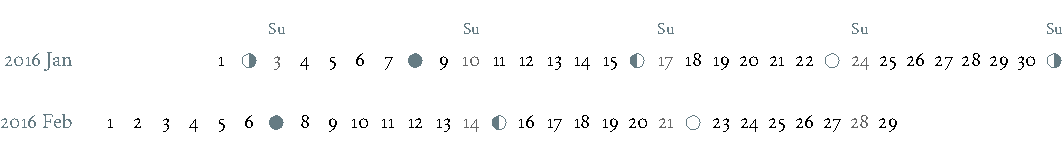
\includegraphics[width=\linewidth]{two-months.pdf}

Keep alternating 30 and 29 day months. One season is four months, one year is
three seasons: Cold-, Hot- and Rainy Season. See Table \ref{tbl-month-names} for
the Pāli names of months and seasons.

\subsection{Marking the Vassa and Major Moondays}
\label{sec-1-2-2}

Mark the months and seasons according to Table \ref{tbl-month-names}.

The key annual events are:

\begin{center}
\begin{tabular}{lll}
 & Lunar Month & \\
Māgha Pūjā & 3rd & \\
Visākha Pūjā & 6th & \\
Āsāḷha Pūjā & 8th & Entering Vassa on the next day\\
Assayuja Pūjā & 11th & Pavāraṇā Day, the end of Vassa\\
\end{tabular}
\end{center}

In a common year, the calendar is finished. 

\subsection{Pāṭimokka announcement}
\label{sec-1-2-3}

TODO

\section{Adhikamāsa year}
\label{sec-1-3}
\subsection{Marking the Vassa and Major Moondays}
\label{sec-1-3-1}

The extra month is a 30 day month. There is a Pali and a Thai method for
inserting it and both are used in the same calendar!

We're gonna need some tables.

The Pali method adds it at different places in different years, see Table
\ref{tbl-cycle-adhikamasa}.

The Thai method always adds it as the month before the Vassa. The convention is
to call this the `second 8th' or `second Āsāḷha', marked as 8/8.

The Major Moondays and the Pāṭimokka announcement of the seasons shift according
to the Pali method, but the beginning of the Vassa, the names of months and
seasons in the calendar are marked according to the Thai method.

In adhikamāsa years the Vassa starts 30 days later, after the 2nd
Āsāḷha, on the day after the Full Moon uposatha of 8/8.

Table \ref{tbl-common-year} shows a common year. Alternating 30 and 29 day
months, three seasons, four months per season.

\begin{table}[p]
\caption{\label{tbl-common-year} Uposathas in a Common Year}
\centering
\begin{tabular}{rrllrl}
1 & 30 &  & New & 1 & Hemanta\\
 &  &  & Full & 2 & \\
2 & 29 &  & New & 3 & \\
 &  &  & Full & 4 & \\
3 & 30 &  & New & 5 & \\
 &  & Māgha & Full & 6 & \\
4 & 29 &  & New & 7 & \\
 &  &  & Full & 8 & \\
\hline
5 & 30 &  & New & 1 & Gimha\\
 &  &  & Full & 2 & \\
6 & 29 &  & New & 3 & \\
 &  & Visākha & Full & 4 & \\
7 & 30 &  & New & 5 & \\
 &  &  & Full & 6 & \\
8 & 29 &  & New & 7 & \\
 &  & Āsāḷha & Full & 8 & \\
\hline
9 & 30 & Enter Vassa & New & 1 & Vassāna\\
 &  &  & Full & 2 & \\
10 & 29 &  & New & 3 & \\
 &  &  & Full & 4 & \\
11 & 30 &  & New & 5 & \\
 &  & Pavāraṇā & Full & 6 & \\
12 & 29 &  & New & 7 & \\
 &  &  & Full & 8 & \\
\end{tabular}
\end{table}

Table \ref{tbl-uposathas-2015} shows the 2015 adhikamāsa year. Looking at Table
\ref{tbl-cycle-adhikamasa} we see that the adhikamāsa is added:

\begin{itemize}
\item in the Rainy Season
\item the first uposatha of the 5-month season is the New Moon of the 9th month (now as 8/8)
\item its last uposatha is the Full Moon of the 12th month
\end{itemize}

\begin{table}[p]
\caption{\label{tbl-uposathas-2015} Uposathas in 2015 with an adhikamāsa}
\centering
\begin{tabular}{rrll|rl|rl}
 &  &  &  &  & Thai &  & Pali\\
\hline
1 & 30 & 2014 Nov 21 & New & 1 & Hemanta & 1 & Hemanta\\
 &  &  & Full & 2 &  & 2 & \\
2 & 29 &  & New & 3 &  & 3 & \\
 &  & 2015 Jan 4 & Full & 4 &  & 4 & \\
3 & 30 &  & New & 5 &  & 5 & \\
 &  &  & Full & 6 &  & 6 & \\
4 & 29 &  & New & 7 &  & 7 & \\
 &  & Māgha & Full & 8 &  & 8 & \\
\hline
5 & 30 &  & New & 1 & Gimha & 1 & Gimha\\
 &  &  & Full & 2 &  & 2 & \\
6 & 29 &  & New & 3 &  & 3 & \\
 &  & Visākha & Full & 4 &  & 4 & \\
7 & 30 &  & New & 5 &  & 5 & \\
 &  &  & Full & 6 &  & 6 & \\
8 & 29 &  & New & 7 &  & 7 & \\
 &  & Āsāḷha & Full & 8 &  & 8 & \\
\hline
8/8 & 30 & 2nd Āsāḷha & New & 9 &  & 1 & Vassāna\\
 &  &  & Full & 10 &  & 2 & \\
\hline
9 & 30 & Enter Vassa & New & 1 & Vassāna & 3 & \\
 &  &  & Full & 2 &  & 4 & \\
10 & 29 &  & New & 3 &  & 5 & \\
 &  &  & Full & 4 &  & 6 & \\
11 & 30 &  & New & 5 &  & 7 & \\
 &  & Pavāraṇā & Full & 6 &  & 8 & \\
12 & 29 &  & New & 7 &  & 9 & \\
 &  &  & Full & 8 &  & 10 & \\
\end{tabular}
\end{table}

Table \ref{tbl-uposathas-2015} shows the 2012 adhikamāsa year. The adhikamāsa is
added:

\begin{itemize}
\item in the Cold Season
\item the first uposatha of the 5-month season is the New Moon of the 1st month
\item its last uposatha is the Full Moon of the 5th month
\end{itemize}

\begin{table}[p]
\caption{\label{tbl-uposathas-2012} Uposathas in 2012 with an adhikamāsa}
\centering
\begin{tabular}{rrll|rl|rl}
 &  &  &  &  & Thai &  & Pali\\
\hline
1 & 30 & 2011 Nov 25 & New & 1 & Hemanta & 1+ & Hemanta\\
 &  &  & Full & 2 &  & 2+ & \\
2 & 29 &  & New & 3 &  & 3 & \\
 &  & 2012 Jan 8 & Full & 4 &  & 4 & \\
3 & 30 &  & New & 5 &  & 5 & \\
 &  &  & Full & 6 &  & 6 & \\
4 & 29 &  & New & 7 &  & 7 & \\
 &  & Māgha & Full & 8 &  & 8 & \\
\hline
5 & 30 &  & New & 1 & Gimha & 9 & \\
 &  &  & Full & 2 &  & 10 & \\
6 & 29 &  & New & 3 &  & 1 & Gimha\\
 &  &  & Full & 4 &  & 2 & \\
7 & 30 &  & New & 5 &  & 3 & \\
 &  & Visākha & Full & 6 &  & 4 & \\
8 & \textbf{30} & 30? & New & 7 &  & 5 & \\
 &  &  & Full & 8 &  & 6 & \\
\hline
8/8 & 30 &  & New & 9+ &  & 7 & \\
 &  & Āsāḷha & Full & 10+ &  & 8 & \\
\hline
9 & 30 & Enter Vassa & New & 1 & Vassāna & 1 & Vassāna\\
 &  &  & Full & 2 &  & 2 & \\
10 & 29 &  & New & 3 &  & 3 & \\
 &  &  & Full & 4 &  & 4 & \\
11 & 30 &  & New & 5 &  & 5 & \\
 &  & Pavāraṇā & Full & 6 &  & 6 & \\
12 & 29 &  & New & 7 &  & 7 & \\
 &  &  & Full & 8 &  & 8 & \\
\end{tabular}
\end{table}

\section{Adhikavāra year}
\label{sec-1-4}

The extra day is inserted in the 8th month (Āsāḷha), making the 7th uposatha of
the Hot Season a 15-day uposatha instead of the expected 14-day, and making
Āsāḷha a 30-day month that year.\cite{hasapannyo-zodiac}

In adhikavāra years the Vassa starts one day later.

\begin{center}
\begin{tabular}{rlr}
order & name & days\\
\hline
6 & Visākha & 29\\
7 & Jeṭṭha & 30\\
8 & Āsāḷha & \textbf{30}\\
9 & Savaṇa & 30\\
10 & Bhaddapāda & 29\\
\end{tabular}
\end{center}

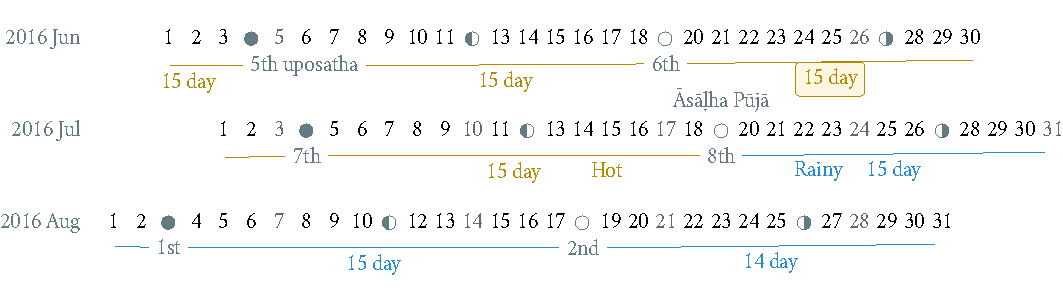
\includegraphics[width=\linewidth]{adding-the-extra-day.pdf}

\clearpage

\chapter{Thailand, Mahānikāya Method}
\label{sec-2}
\section{Adding the extra month}
\label{sec-2-1}

The extra month (adhikamāsa) is added 7 times in every 19 year, in a repeating
pattern of 3-3-2 - 3-3-3-2 years. This is a shorthand for the formulas
at \ref{fig-suriyayatra} which generate this pattern. Table
\ref{tbl-cycle-adhikamasa} shows adhikamāsa years for 1996-2034.

In Thai practice, the extra month is a 30 day month inserted after the
8th month (\emph{Āsāḷha}), at the end of the Hot Season. The convention is
to call this the `second 8th' or `second \emph{Āsāḷha}', marked as 8/8.

In adhikamāsa years the Vassa starts 30 days later, after the 2nd
Āsāḷha, on the day after the Full Moon uposatha of 8/8.

\begin{center}
\begin{tabular}{rlr}
order & name & days\\
\hline
8 & Āsāḷha & 29\\
8/8 & 2nd Āsāḷha & 30\\
9 & Savaṇa & 30\\
\end{tabular}
\end{center}
\section{Adding the extra day}
\label{sec-2-2}
\label{adding-extra-day}

The extra day (adhikavāra) is added 11 times in every 57 year.

Whether a year should have an extra day can be determined with the
conditions at sec.\ref{adhikawan-years}.

In Thai practice a year with an extra month is not allowed to also
have an extra day. If the year should have an extra day, but it
already has an extra month, the extra day is assigned to one of the
flanking years (next or previous, in the case of planning several
years in advance).

In adhikavāra years the Vassa starts one day later.

If the year is going to have an extra day, it is inserted in the 8th month
(Āsāḷha), making the 7th uposatha of the Hot Season a 15-day uposatha instead of
the expected 14-day, and making Āsāḷha a 30-day month that
year.\cite{hasapannyo-zodiac}

\begin{center}
\begin{tabular}{rlr}
order & name & days\\
\hline
6 & Visākha & 29\\
7 & Jeṭṭha & 30\\
8 & Āsāḷha & \textbf{30}\\
9 & Savaṇa & 30\\
10 & Bhaddapāda & 29\\
\end{tabular}
\end{center}

However, this is the most unpredictable variable in the calendars
published for a given year, and the various calendar authorities add
the extra day in a flexible manner, in some of cases according with
the formula but differing from it in others.

Nonetheless they observe that:

\begin{itemize}
\item the count for 11 times in 57 years is maintained to keep the
calendar at pace
\item the extra day will not be in years that also have an extra month.
\end{itemize}

\begin{table}[p]
\caption{\label{tbl-cycle-adhikavara} Adhikavāra years}\legend{K, A, T for kammacubala, avoman and thaloengsok}
\centering
\begin{tabular}{rrrrr}
Year & CS & K & A & T\\
\hline
1994 & 1356 & 535 & 54 & 6\\
2000 & 1362 & 93 & 627 & 11\\
2005 & 1367 & 658 & 656 & 7\\
2009 & 1371 & 630 & 119 & 22\\
2014 & 1376 & 395 & 137 & 17\\
2016 & 1378 & 781 & 566 & 9\\
2020 & 1382 & 753 & 29 & 24\\
2025 & 1387 & 518 & 47 & 19\\
\end{tabular}
\end{table}

\subsection{Check: Adhikavāra prediction}
\label{sec-2-2-1}
\label{adhikavara-prediction}

The formulas predict 2016 to have an adhikavāra. See below for the
\emph{kammacubala} (K), \emph{avoman} (A) and \emph{thaloengsok} (T) values produced
with the formulas \ref{fig-suriyayatra}.

See description at sec.\ref{adhikamat-years} and
sec.\ref{adhikawan-years}.

The last adhikavāra year has been 2009, which makes 2016 a likely
candidate. If relatively evenly distributed, the adhikavāra years are
5-6 years in distance, and 2015 would have probably been adhikavāra if
not for the adhikamāsa.

2015 qualifies for adhikamat, but also for adhikawan, and so the
adhikawan would be carried on to 2016.

\begin{center}
\begin{tabular}{rrlrrr}
AD & CS & type & K & A & T\\
2015 & 1377 & m & 188 & 0 & 28\\
2016 & 1378 & d & 781 & 566 & 9\\
\end{tabular}
\end{center}

\section{Major Moondays}
\label{sec-2-3}
\label{major-moondays}

Buddhist communities observe key annual events on the Full Moon
days of four lunar months:

\begin{center}
\begin{tabular}{lll}
 & Lunar Month & \\
Māgha Pūjā & 3rd & \\
Visākha Pūjā & 6th & \\
Āsāḷha Pūjā & 8th & Entering Vassa on the next day\\
Assayuja Pūjā & 11th & Pavāraṇā Day, the end of Vassa\\
\end{tabular}
\end{center}

The Pāli method for adding the adhikamāsa at sec.\ref{pali-method} is
relevant here.

In adhikamāsa years the extra month is added as the 2nd Āsāḷha, but
the numbering of months for determining the major moondays moves
forward as if it was added in the season described by the Pāli method.

If the adhikamāsa falls in the Cold Season, the Sangha still observes
it in that season when telling the season at the recitation of the
Pāṭimokkha.

Also see sec.\ref{lunar-month-first-last} on \emph{Thai} lunar months.

\clearpage
\chapter{Adding the extra month, Pali method}
\label{sec-3}
\label{pali-method}

\emph{The following is adapted from Ajahn Khemanando for recent
years.}\cite{khemanando-adhikamasa}

Table \ref{tbl-cycle-adhikamasa} shows the 19-year cycle between
1996-2034.

\begin{table}[h]
\caption{\label{tbl-cycle-adhikamasa} Adhikamāsa years for 1996-2034 and inserting the extra month according to Pali method.}\legend{\Delta m for years since last adhikamāsa.}
\centering
\begin{tabular}{rrrr|rlrr}
$\Delta$ m &  &  &  & Month & Season & New & Full\\
\hline
 & 0 & 1996 & 2015 & 8 & Rainy & 9 & 12\\
 & 1 &  &  &  &  &  & \\
 & 2 &  &  &  &  &  & \\
3 & 3 & 1999 & 2018 & 5 & Hot & 5 & 8/8\\
 & 4 &  &  &  &  &  & \\
 & 5 &  &  &  &  &  & \\
3 & 6 & 2002 & 2021 & 2 & Cold & 1 & 5\\
 & 7 &  &  &  &  &  & \\
2 & 8 & 2004 & 2023 & 10 & Rainy & 9 & 12\\
 & 9 &  &  &  &  &  & \\
 & 10 &  &  &  &  &  & \\
3 & 11 & 2007 & 2026 & 7 & Hot & 5 & 8/8\\
 & 12 &  &  &  &  &  & \\
 & 13 &  &  &  &  &  & \\
3 & 14 & 2010 & 2029 & 3 & Cold & 1 & 5\\
 & 15 &  &  &  &  &  & \\
2 & 16 & 2012 & 2031 & 12 & Cold & 1 & 5\\
 & 17 &  &  &  &  &  & \\
 & 18 &  &  &  &  &  & \\
3 & 19 & 2015 & 2034 & 8 & Rainy & 9 & 12\\
\end{tabular}
\end{table}

\begin{description}
\item[{$\Delta$ m:}] years since the last adhikamāsa
\item[{Month:}] the Pali lunar month into which the adhikamāsa is inserted
\item[{Season:}] the season in which the adhikamāsa falls in that particular year
\item[{New and Full:}] the first and last uposatha of the 5-month season in which
the adhikamāsa falls, numbered in Pali lunar months
\end{description}

If the adhikamāsa falls on the 2nd, 3rd, or 12th Pali lunar month,
there will be \emph{two} 8th months (8 and 8/8) the following year.

E.g. In 2001, the adhikamāsa comes as the 2nd lunar month in the
Cold Season, so the following year, 2002, has two 8th months (8 and
8/8). There will thus be \emph{ten} uposathas in the Cold Season, the
first being the New Moon of the 1st Pali lunar month (2002) and the
last being the Full Moon of the 5th Pali lunar month, 2002.

\clearpage
\chapter{The Thai luni-solar calendar}
\label{sec-4}

Luni-solar calendars are constructed so to count years according to
the \emph{solar} cycle, but to count months according to the \emph{lunar} cycle.

\begin{center}
\begin{tabular}{ll}
tropical year\footnotemark\space of the Earth & 365.24219 days\\
synodic month\footnotemark\space of the Moon & \textasciitilde{}29.53 days, can vary up to 7 hours\\
\end{tabular}
\end{center}\footnotetext[1]{tropical year: the time it takes the Earth to
complete an orbit around the Sun}\footnotetext[2]{synodic month: the time it takes the Moon to reach
the same visual phase

\clearpage}

The epoch of the Thai calendar is 25 March 638 AD.

The Thai luni-solar calendar is \emph{procedural}, it uses a few constant,
key numbers derived from astronomical observations, and applies a
series of mechanical calculations (i.e. the ``rules'') again and again
to generate the dates of lunar phases and new years.

\begin{quote}
This working is deliberately concise, since it thereby reflects how
the calculation would have been made by a South East Asian calendrist.
Each stage is subjected to an operation learnt by rote, and the
underlying theory disappears from view. The rote operations, however,
will provide a valid answer for any date in any year. It seemed
greatly preferable to set out the procedure thus starkly, rather than
to give a detailed exposition of what is involved.\cite{eade-interpolation}
\end{quote}

Southeast Asian astronomers refined a fraction to obtain the length of
the year:

\begin{equation}
\frac{292207}{800} = 365.25875\ \text{days}\cite{eade-interpolation}
\end{equation}

This is 0.01656 days longer than the modern measurement (accumulating
1 day in \textasciitilde{}60 years). Remarkably, the \emph{suriyayatra} accounts for this
and generates accurate results:

\begin{quote}
For instance, a Pagan inscription of 14 April 1288 AD maintains that
at midnight the Sun's position was 0 signs, 19 degrees and 59 minutes:
the computer program returns
0~19~59.\cite{eade-calendrical}
\end{quote}

Nonetheless, the calendar dates published in Thailand (historical or
recent) in a given year reflect not only these principles, but also
adjustments and omissions which cannot be foreseen or retraced.

\begin{quote}
The historical record however, frequently defies prediction, forcing
the conclusion that the pressure upon the \emph{horas} (astronomers /
astrologers) was not to follow the ``rules'' but merely, within some
more leisurely constraints, to ensure that the calendar did not get
out of control.\cite{eade-calendrical}
\end{quote}

\section{Year Types}
\label{sec-4-1}

\begin{multicols}{2}

We are concerned with three types of calendar years:

\begin{description}
\item[{Cal A}] Normal with 354 days
\item[{Cal B}] Adhikavāra with 355 days
\item[{Cal C}] Adhikamāsa with 384 days
\end{description}

\columnbreak

Comparing these to normal and solar leap years:

\begin{center}
\begin{tabular}{lrrr}
 & A & B & C\\
Lunar & 354 & 355 & 384\\
Solar & 365 & 365 & 365\\
difference & +11 & +10 & -19\\
\hline
 & A & B & C\\
Lunar & 354 & 355 & 384\\
Solar Leap & 366 & 366 & 366\\
difference & +12 & +11 & -18\\
\end{tabular}
\end{center}

\end{multicols}

\section{The first and last day of a lunar month}
\label{sec-4-2}
\label{lunar-month-first-last}

In monastic practice, the Full Moon day is on the last day of a given
month. The next month starts on the following day (first day of the
waning phase), thus the first uposatha will be on a New Moon.

In many Thai calendars, the New Moon day is the last day of the month,
and the Full Moon day is in the middle. This only changes the
numbering of the months, not the actual moondays. In these calendars
the thresholds of months are shifted two weeks forward relative to the
monastic calendar.

The New Moon of the 7th \emph{Thai} lunar month is the New Moon (1st
uposatha) of the 8th \emph{monastic} lunar month.

\begin{table}[p]
\caption{\label{pali-thai-year} Pali and Thai lunar months in a year}
\centering
\begin{tabular}{rllrr}
Nth & phase & month & Pali & Thai\\
\hline
1 & New &  & 1 & 12\\
2 & Full &  & 1 & 1\\
3 & New &  & 1 & 1\\
4 & Full & Magasira & 1 & 1\\
5 & New &  & 2 & 1\\
6 & Full &  & 2 & 2\\
7 & New &  & 2 & 2\\
8 & Full & Phussa & 2 & 2\\
9 & New &  & 3 & 2\\
10 & Full &  & 3 & 3\\
11 & New &  & 3 & 3\\
12 & Full & Māgha & 3 & 3\\
13 & New &  & 4 & 3\\
14 & Full &  & 4 & 4\\
\end{tabular}
\end{table}

\section{Adhikamat years}
\label{sec-4-3}
\label{adhikamat-years}

The \emph{suriyayatra} principle to determine adhikamat years is:

\begin{quote}
If the day of \emph{thaloengsok} (astronomical New Year)
lies either within 25 to 29 (in Citta-māsa) or 1 to 5 (in
Visākha-māsa), then the year is adhikamat.\cite{prasert-ngan}
\end{quote}

The \emph{thaloengsok} is the value of T in Figure \ref{fig-suriyayatra}.

\section{Adhikawan years}
\label{sec-4-4}
\label{adhikawan-years}

\begin{quote}
Two components of the \emph{suriyayatra} are known as the \emph{kammacubala} and
the \emph{avoman}, and it is the values of these two elements at the start
of the year that determine the matter:

\begin{itemize}
\item if the kammacubala value is 207 or less, then the year is leap year
\item in a leap year, if the avoman is 126 or less, the year will have an
extra day
\item in a normal year, if the avoman is 137 or less, the year will have
and extra day\cite{eade-interpolation}
\end{itemize}
\end{quote}

The \emph{kammacubala} and \emph{avoman} are the value of K and A in Figure
\ref{fig-suriyayatra}.

In Thailand, years with an extra month are not allowed to also have an
extra day, and the adhikawan will be assigned to the previous or next
year.

\section{Suriyayatra formulas}
\label{sec-4-5}

See Figure \ref{fig-suriyayatra}.

\begin{figure}
\caption{\label{fig-suriyayatra}Finding astronomical values with the \emph{suriyayatra} calculation\cite{eade-interpolation}}
\legend{Start with Y, the given Common Era year. Significant values are assigned names. K for \emph{kammacubala}, A for \emph{avoman}, T for \emph{thaloengsok} (the New Year).}
\begin{eqnarray}
a & = & ((Y - 638) * 292207) + 373 \\
h & = & \lfloor a/800 + 1 \rfloor \\
K & = & 800 - (a \bmod 800) \\
A & = & ((h*11) + 650) \bmod 692 \\
b & = & \lfloor ((h*11) + 650) / 692 \rfloor \\
T & = & (b + h) \bmod 30
\end{eqnarray}
\end{figure}

\begin{table}[p]
\caption{Adhikamat and adhikawan in the period 1958 to 1978 (CS 1320-1340).\cite{eade-interpolation}}\legend{m for adhikamat, d for adhikawan years, \Delta m and \Delta d for years since last adhikamat and adhikawan.}
\centering
\begin{tabular}{rrrrrlrr}
 & $\Delta$ d &  & $\Delta$ m & year & type & Asalha & 2nd Asalha\\
\hline
 &  & 0 &  & 1320 & m & 19:42 & 22:24\\
0 &  & 1 &  & 1321 & d & 21:05 & \\
1 &  & 2 &  & 1322 &  & 20:40 & \\
2 &  & 3 & 3 & 1323 & m & 19:12 & 22:00\\
3 &  & 4 &  & 1324 &  & 20:38 & \\
4 & 4 & 5 &  & 1325 & d & 19:34 & \\
5 &  & 6 & 3 & 1326 & m & 19:38 & 22:05\\
6 &  & 7 &  & 1327 &  & 21:15 & \\
7 &  & 8 & 2 & 1328 & m & 19:20 & 22:55\\
8 &  & 9 &  & 1329 &  & 21:48 & \\
9 & 5 & 10 &  & 1330 & d & 20:26 & \\
10 &  & 11 & 3 & 1331 & m & 19:59 & 22:50\\
11 &  & 12 &  & 1332 &  & 21:20 & \\
12 &  & 13 &  & 1333 &  & 20:02 & \\
13 &  & 14 & 3 & 1334 & m & 19:03 & 21:33\\
14 & 5 & 15 &  & 1335 & d & 20:40 & \\
15 &  & 16 &  & 1336 &  & 20:44 & \\
16 &  & 17 & 3 & 1337 & m & 19:44 & 22:19\\
17 &  & 18 &  & 1338 &  & 21:11 & \\
18 &  & 19 & 2 & 1339 & m & 19:45 & 22:35\\
19 & 5 &  &  & 1340 & d & 21:05 & \\
\end{tabular}
\end{table}
\section{Names of the months}
\label{sec-4-6}

The name of a given month is determined by the astrological sign which
the Full Moon enters at midnight. See Table \ref{tbl-month-names}.

\begin{table}[htb]
\caption{\label{tbl-month-names}Lunar and Solar Months and Zodiacs\cite{hasapannyo-zodiac}}
\centering
\begin{tabular}{lrrlll}
Season &  &  & Lunar Month & Solar Month & Solar Zodiac\\
 &  & days &  &  & (Western / Sanskrit)\\
\hline
Hemanta-utu & 1 & 30 & Magasira-māsa & December & Sagittarius / Dhanus\\
Cold Season & 2 & 29 & Phussa-māsa & January & Capricorn / Makara\\
 & 3 & 30 & Māgha-māsa & February & Aquarius / Kumbha\\
 & 4 & 29 & Phagguṇa-māsa & March & Pisces / Mīna\\
\hline
Gimha-utu & 5 & 30 & Citta-māsa & April & Aries / Meṣa\\
Hot Season & 6 & 29 & Visākha-māsa & May & Taurus / Vṛṣabha\\
 & 7 & 30 & Jeṭṭha-māsa & June & Gemini / Mithuna\\
 & 8 & 29 & Āsāḷha-māsa & July & Cancer / Karkaṭa\\
\hline
Vassāna-utu & 9 & 30 & Savaṇa-māsa & August & Leo / Siṃha\\
Rainy Season & 10 & 29 & Bhaddapāda-māsa & September & Virgo / Kanyā\\
 & 11 & 30 & Assayuja-māsa & October & Libra / Tulā\\
 & 12 & 29 & Kattika-māsa & November & Scorpio / Vṛścika\\
\end{tabular}
\end{table}

\chapter{Gregorian leap years}
\label{sec-5}

\begin{table}[h]
\caption{\label{tbl-cycle-leap-years} Gregorian leap years}
\centering
\begin{tabular}{rrrr}
2004 & 2016 & 2028 & 2040\\
2008 & 2020 & 2032 & 2044\\
2012 & 2024 & 2036 & 2048\\
\end{tabular}
\end{table}

\begin{quote}
\textbf{if} (\emph{year} is not exactly divisible by 4) \textbf{then} (it is a common year)\\
\textbf{else}\\
\textbf{if} (\emph{year} is not exactly divisible by 100) \textbf{then} (it is a leap year)\\
\textbf{else}\\
\textbf{if} (\emph{year} is not exactly divisible by 400) \textbf{then} (it is a common year)\\
\textbf{else} (it is a leap year)
\cite{wp-leap-year}
\end{quote}

\backmatter

\chapter{Bibliography}
\label{sec-6}
\label{bibliography}

\bibliographystyle{plain}
\bibliography{bibentries}
\chapter{Colophon}
\label{sec-7}

\href{http://orgmode.org/}{Org-mode} and \LaTeX. Sources at \href{https://github.com/profound-labs/calculating-the-uposatha-moondays/}{Github}.

Comments, corrections and further information would be greatly
appreciated.

\texttt{Gambhiro Bhikkhu <gambhiro.bhikkhu.85@gmail.com>}

Last updated on 2015-08-04.
% Emacs 25.0.50.1 (Org mode 8.2.10)
\end{document}